\section{Preventivo}
Questa sezione fornisce una stima dei costi che il gruppo dovrà sostenere nelle varie fasi che interessano lo svolgimento del progetto. In particolare, verranno utilizzate le seguenti abbreviazioni per descrivere l'utilizzo delle risorse da parte del team:
\begin{itemize}
	\item R  -> Responsabile
	\item V  -> Verificatore
	\item An -> Analista
	\item Am -> Amministratore
	\item Pr -> Programmatore
	\item Pt -> Progettista
\end{itemize}


\subsection{Avvio}

\subsubsection{Prospetto orario}
Di seguito viene illustrato l'utilizzo della risorsa tempo (espresso in ore) dei vari componenti del gruppo nella fase di Avvio:

\begin{table}[hbt!]
\begin{center}
\begin{tabular}{c
	!{\color[HTML]{9b240a}\vrule width 1pt}
	cccccc
	!{\color[HTML]{9b240a}\vrule width 1pt}	
	c}
\rowcolorhead
\headertitle{Nome} & \headertitle{R} & \headertitle{V} & \headertitle{An} & \headertitle{Am} & \headertitle{Pr} & \headertitle{Pt} & \headertitle{Tot} \\

Chiarello Sofia & 0 & 0 & 0 & 0 & 0 & 0 & 0\\
Crivellari Alberto & 0 & 0 & 0 & 0 & 0 & 0 & 0\\
De Renzis Simone & 0 & 0 & 0 & 0 & 0 & 0 & 0\\
Greggio Nicolò & 0 & 0 & 0 & 0 & 0 & 0 & 0\\
Tessari Andrea & 0 & 0 & 0 & 0 & 0 & 0 & 0\\
Zuccolo Giada & 0 & 0 & 0 & 0 & 0 & 0 & 0\\
\end{tabular}
\caption{Per ogni componente, i ruoli ricoperti e la relativa occupazione oraria nella fase di Avvio}
\end{center}
\end{table}

%%%%%DON'T COPY THIS%%%%%%
\pagebreak
%%%%%DON'T COPY THIS%%%%%%

\begin{figure}[hbt!]
\centering
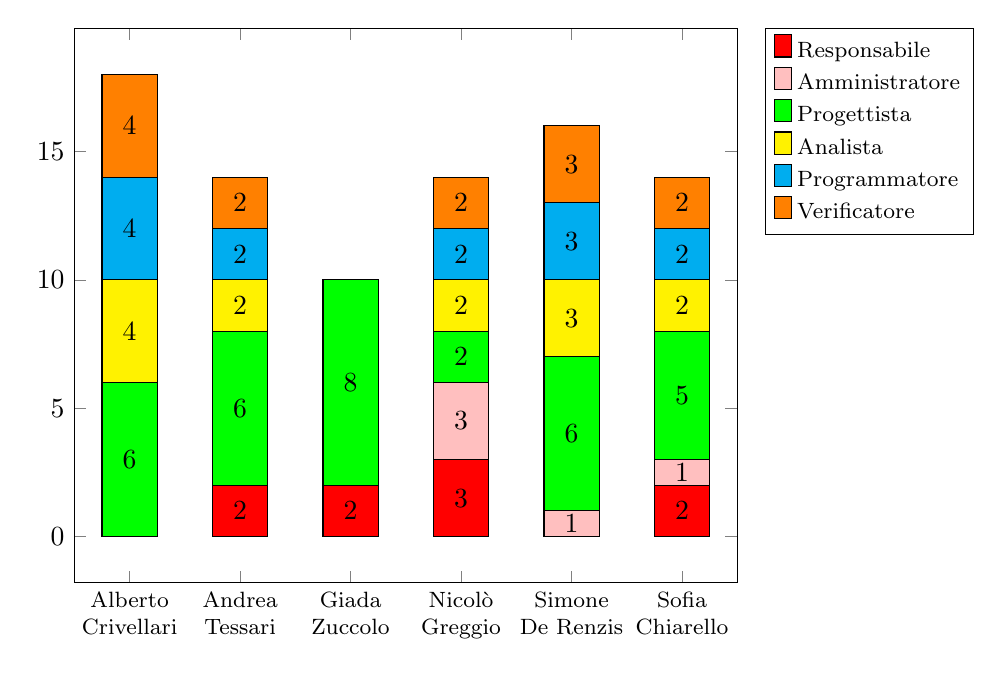
\begin{tikzpicture}
\begin{axis}[
    ybar stacked,
    width=10cm,
    bar width=0.7cm,
    %every node near coord/.style={text width=3 cm},
    nodes near coords,
     every node near coord/.append style={color=black},
    enlargelimits=0.10,
    legend style={font=\footnotesize,at={(1.2,1)},
    cells={anchor=west},
      anchor=north,legend columns=1},
    %ylabel={\#participants},
    symbolic x coords={Alberto Crivellari, Andrea Tessari, Giada Zuccolo, Nicolò Greggio, Simone De Renzis, Sofia Chiarello},
    xtick=data,
    x tick label style={font=\footnotesize,text width=1.7cm,align=center},
    ]
\addplot+[ybar,fill=red, draw=black] plot coordinates {(Alberto Crivellari,0) (Andrea Tessari,2) 
  (Giada Zuccolo,2) (Nicolò Greggio,3) (Simone De Renzis,0) (Sofia Chiarello,2) };
\addplot+[ybar,fill=pink, draw=black] plot coordinates {(Alberto Crivellari,0) (Andrea Tessari,0) 
  (Giada Zuccolo,0) (Nicolò Greggio,3) (Simone De Renzis,1) (Sofia Chiarello,1) };
\addplot+[ybar,fill=green, draw=black] plot coordinates {(Alberto Crivellari,6) (Andrea Tessari,6)
  (Giada Zuccolo,8) (Nicolò Greggio,2) (Simone De Renzis,6) (Sofia Chiarello,5) };
\addplot+[ybar,fill=yellow, draw=black] plot coordinates {(Alberto Crivellari,4) (Andrea Tessari,2) 
  (Giada Zuccolo,0) (Nicolò Greggio,2) (Simone De Renzis,3) (Sofia Chiarello,2) };
\addplot+[ybar,fill=cyan, draw=black] plot coordinates {(Alberto Crivellari,4) (Andrea Tessari,2) 
  (Giada Zuccolo,0) (Nicolò Greggio,2) (Simone De Renzis,3) (Sofia Chiarello,2) };
\addplot+[ybar,fill=orange, draw=black] plot coordinates {(Alberto Crivellari,4) (Andrea Tessari,2) 
  (Giada Zuccolo,0) (Nicolò Greggio,2) (Simone De Renzis,3) (Sofia Chiarello,2) };
\legend{Responsabile \\ Amministratore \\ Progettista \\ Analista \\ Programmatore \\ Verificatore \\}
\end{axis}
\end{tikzpicture}
\caption{Istogramma che visualizza la ripartizione delle ore per la fase di Avvio} 
\end{figure}







\subsubsection{Prospetto economico}
Il costo derivante dalle ore impiegate dai componenti è descritto di seguito, calcolandone il totale.

\begin{table}[hbt!]
{\setlength{\parindent}{0cm}
\begin{minipage}{.43\textwidth}
	\begin{tabular}{ccc}
	\rowcolorhead
	\headertitle{Ruolo} & \headertitle{Ore} & \headertitle{Costo(€)}\\
	Responsabile & 0 & 0\\
	Verificatore & 0 & 0\\
	Analista & 0 & 0\\
	Programmatore & 0 & 0\\
	Progettista & 0 & 0\\
	\hline
	Totale & 0& 0\\
	\end{tabular}
\end{minipage}% This must go next to `\end{minipage}`
\begin{minipage}{.57\textwidth}
  \begin{tikzpicture}
\pie [rotate = 270,
    sum = auto, 
    %text = legend, 
    radius = 2.7,
    color = {red, pink, green, yellow, cyan, orange}]
    {
    20/Responsabile,
    65/Amministratore,
    5/Progettista,
    15/Analista,
    3/Programmatore,
	15/Verificatore
    }
\end{tikzpicture} 
\end{minipage} }
\caption{Per ogni ruolo, il complessivo delle ore impiegate dai membri e il relativo ammontare in denaro. Il diagramma a torta visualizza la composizione del costo per la fase di Avvio}
\end{table}



\subsection{Analisi dei requisiti}

\subsubsection{Prospetto orario}
Questa tabella descrive l'utilizzo della risorsa tempo (in ore) dei vari componenti del gruppo in questa fase: \\

\begin{tabular}{|l|cccccc|c|}
\hline
Nome & R &  V & An & Am & Pr & Pt & Tot(h)\\
\hline
Chiarello Sofia & 0 & 0 & 0 & 0 & 0 & 0 & 0\\
Crivellari Alberto & 0 & 0 & 0 & 0 & 0 & 0 & 0\\
De Renzis Simone & 0 & 0 & 0 & 0 & 0 & 0 & 0\\
Greggio Nicolò & 0 & 0 & 0 & 0 & 0 & 0 & 0\\
Tessari Andrea & 0 & 0 & 0 & 0 & 0 & 0 & 0\\
Zuccolo Giada & 0 & 0 & 0 & 0 & 0 & 0 & 0\\
\hline
\end{tabular}
\\
Vengono riportati i dati della tabella nel seguente istogramma: \\

\pgfplotsset{width=10cm,compat=1.17}

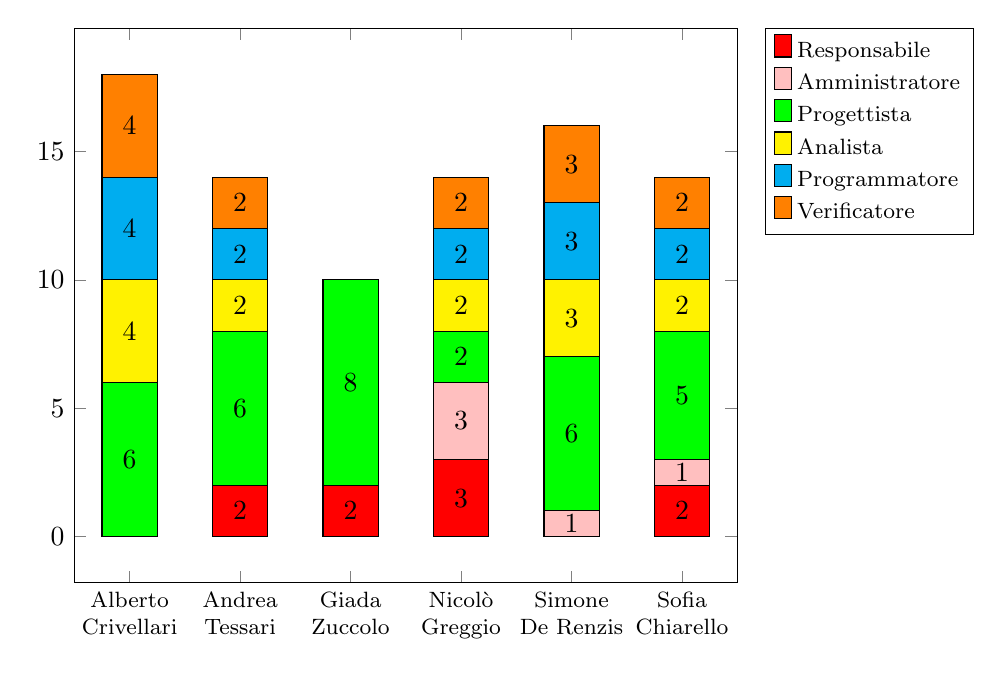
\begin{tikzpicture}
\begin{axis}[
    ybar stacked,
    width=10cm,
    bar width=0.7cm,
    %every node near coord/.style={text width=3 cm},
    nodes near coords,
     every node near coord/.append style={color=black},
    enlargelimits=0.10,
    legend style={font=\footnotesize,at={(1.2,1)},
    cells={anchor=west},
      anchor=north,legend columns=1},
    %ylabel={\#participants},
    symbolic x coords={Alberto Crivellari, Andrea Tessari, Giada Zuccolo, Nicolò Greggio, Simone De Renzis, Sofia Chiarello},
    xtick=data,
    x tick label style={font=\footnotesize,text width=1.7cm,align=center},
    ]
\addplot+[ybar,fill=red, draw=black] plot coordinates {(Alberto Crivellari,0) (Andrea Tessari,2) 
  (Giada Zuccolo,2) (Nicolò Greggio,3) (Simone De Renzis,0) (Sofia Chiarello,2) };
\addplot+[ybar,fill=pink, draw=black] plot coordinates {(Alberto Crivellari,0) (Andrea Tessari,0) 
  (Giada Zuccolo,0) (Nicolò Greggio,3) (Simone De Renzis,1) (Sofia Chiarello,1) };
\addplot+[ybar,fill=green, draw=black] plot coordinates {(Alberto Crivellari,6) (Andrea Tessari,6)
  (Giada Zuccolo,8) (Nicolò Greggio,2) (Simone De Renzis,6) (Sofia Chiarello,5) };
\addplot+[ybar,fill=yellow, draw=black] plot coordinates {(Alberto Crivellari,4) (Andrea Tessari,2) 
  (Giada Zuccolo,0) (Nicolò Greggio,2) (Simone De Renzis,3) (Sofia Chiarello,2) };
\addplot+[ybar,fill=cyan, draw=black] plot coordinates {(Alberto Crivellari,4) (Andrea Tessari,2) 
  (Giada Zuccolo,0) (Nicolò Greggio,2) (Simone De Renzis,3) (Sofia Chiarello,2) };
\addplot+[ybar,fill=orange, draw=black] plot coordinates {(Alberto Crivellari,4) (Andrea Tessari,2) 
  (Giada Zuccolo,0) (Nicolò Greggio,2) (Simone De Renzis,3) (Sofia Chiarello,2) };
\legend{Responsabile \\ Amministratore \\ Progettista \\ Analista \\ Programmatore \\ Verificatore \\}
\end{axis}
\end{tikzpicture}

\subsubsection{Prospetto economico}
Questa tabella mostra il costo per ogni ruolo all'interno del team in questa fase. Viene mostrato anche il totale. \\

\begin{tabular}{ccc}
\rowcolorhead
\headertitle{Ruolo} & \headertitle{Ore} & \headertitle{Costo(€)}\\
Responsabile & 0 & 0\\
Verificatore & 0 & 0\\
Analista & 0 & 0\\
Programmatore & 0 & 0\\
Progettista & 0 & 0\\
Totale & 0& 0\\
\end{tabular}\\

Vengono riportati i dati della tabella nel seguente grafico a torta: \\

\begin{tikzpicture}
\pie [rotate = 180, sum = auto, explode=0.1]
    {
    20/Responsabile,
	15/Verficatore,
	15/Analista,
	65/Amministratore,
	3/Programmatore,
	5/Progettista
    }
\end{tikzpicture}

\subsection{Progettazione architetturale}

\subsubsection{Prospetto orario}
Questa tabella descrive l'utilizzo della risorsa tempo (in ore) dei vari componenti del gruppo in questa fase: \\

\begin{tabular}{|l|cccccc|c|}
\hline
Nome & R &  V & An & Am & Pr & Pt & Tot(h)\\
\hline
Chiarello Sofia & 0 & 0 & 0 & 0 & 0 & 0 & 0\\
Crivellari Alberto & 0 & 0 & 0 & 0 & 0 & 0 & 0\\
De Renzis Simone & 0 & 0 & 0 & 0 & 0 & 0 & 0\\
Greggio Nicolò & 0 & 0 & 0 & 0 & 0 & 0 & 0\\
Tessari Andrea & 0 & 0 & 0 & 0 & 0 & 0 & 0\\
Zuccolo Giada & 0 & 0 & 0 & 0 & 0 & 0 & 0\\
\hline
\end{tabular}
\\
Vengono riportati i dati della tabella nel seguente istogramma: \\

\pgfplotsset{width=10cm,compat=1.17}

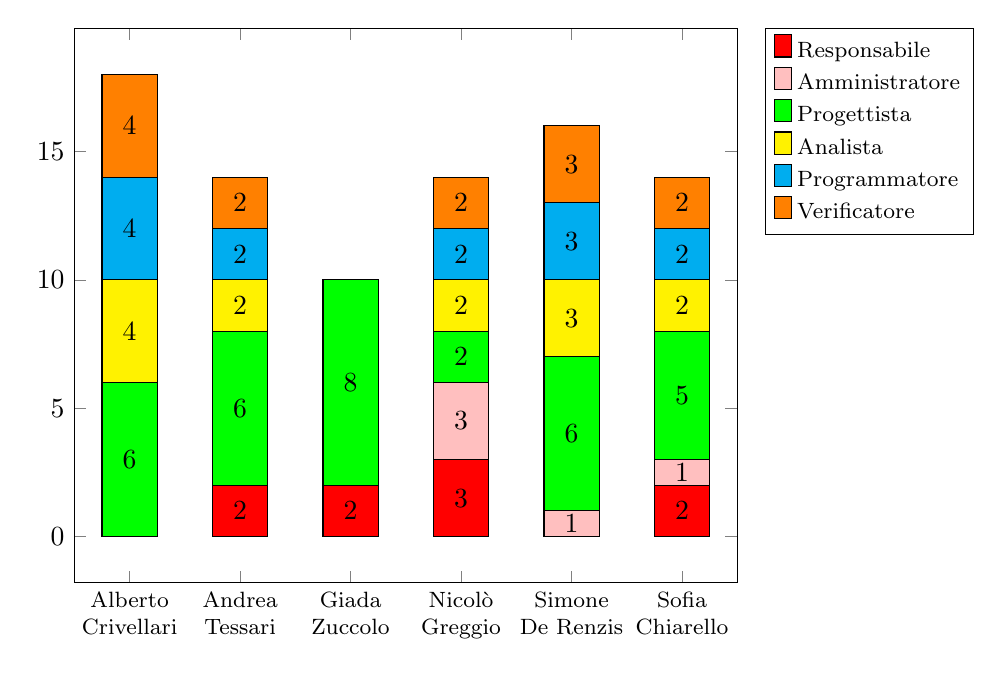
\begin{tikzpicture}
\begin{axis}[
    ybar stacked,
    width=10cm,
    bar width=0.7cm,
    %every node near coord/.style={text width=3 cm},
    nodes near coords,
     every node near coord/.append style={color=black},
    enlargelimits=0.10,
    legend style={font=\footnotesize,at={(1.2,1)},
    cells={anchor=west},
      anchor=north,legend columns=1},
    %ylabel={\#participants},
    symbolic x coords={Alberto Crivellari, Andrea Tessari, Giada Zuccolo, Nicolò Greggio, Simone De Renzis, Sofia Chiarello},
    xtick=data,
    x tick label style={font=\footnotesize,text width=1.7cm,align=center},
    ]
\addplot+[ybar,fill=red, draw=black] plot coordinates {(Alberto Crivellari,0) (Andrea Tessari,2) 
  (Giada Zuccolo,2) (Nicolò Greggio,3) (Simone De Renzis,0) (Sofia Chiarello,2) };
\addplot+[ybar,fill=pink, draw=black] plot coordinates {(Alberto Crivellari,0) (Andrea Tessari,0) 
  (Giada Zuccolo,0) (Nicolò Greggio,3) (Simone De Renzis,1) (Sofia Chiarello,1) };
\addplot+[ybar,fill=green, draw=black] plot coordinates {(Alberto Crivellari,6) (Andrea Tessari,6)
  (Giada Zuccolo,8) (Nicolò Greggio,2) (Simone De Renzis,6) (Sofia Chiarello,5) };
\addplot+[ybar,fill=yellow, draw=black] plot coordinates {(Alberto Crivellari,4) (Andrea Tessari,2) 
  (Giada Zuccolo,0) (Nicolò Greggio,2) (Simone De Renzis,3) (Sofia Chiarello,2) };
\addplot+[ybar,fill=cyan, draw=black] plot coordinates {(Alberto Crivellari,4) (Andrea Tessari,2) 
  (Giada Zuccolo,0) (Nicolò Greggio,2) (Simone De Renzis,3) (Sofia Chiarello,2) };
\addplot+[ybar,fill=orange, draw=black] plot coordinates {(Alberto Crivellari,4) (Andrea Tessari,2) 
  (Giada Zuccolo,0) (Nicolò Greggio,2) (Simone De Renzis,3) (Sofia Chiarello,2) };
\legend{Responsabile \\ Amministratore \\ Progettista \\ Analista \\ Programmatore \\ Verificatore \\}
\end{axis}
\end{tikzpicture}

\subsubsection{Prospetto economico}
Questa tabella mostra il costo per ogni ruolo all'interno del team in questa fase. Viene mostrato anche il totale. \\

\begin{tabular}{ccc}
\rowcolorhead
\headertitle{Ruolo} & \headertitle{Ore} & \headertitle{Costo(€)}\\
Responsabile & 0 & 0\\
Verificatore & 0 & 0\\
Analista & 0 & 0\\
Programmatore & 0 & 0\\
Progettista & 0 & 0\\
Totale & 0& 0\\
\end{tabular}\\

Vengono riportati i dati della tabella nel seguente grafico a torta: \\

\begin{tikzpicture}
\pie [rotate = 180, sum = auto, explode=0.1]
    {
    20/Responsabile,
	15/Verficatore,
	15/Analista,
	65/Amministratore,
	3/Programmatore,
	5/Progettista
    }
\end{tikzpicture}


\subsection{Progettazione di dettaglio e codifica}

\subsubsection{Prospetto orario}
Questa tabella descrive l'utilizzo della risorsa tempo (in ore) dei vari componenti del gruppo in questa fase: \\

\begin{tabular}{|l|cccccc|c|}
\hline
Nome & R &  V & An & Am & Pr & Pt & Tot(h)\\
\hline
Chiarello Sofia & 0 & 0 & 0 & 0 & 0 & 0 & 0\\
Crivellari Alberto & 0 & 0 & 0 & 0 & 0 & 0 & 0\\
De Renzis Simone & 0 & 0 & 0 & 0 & 0 & 0 & 0\\
Greggio Nicolò & 0 & 0 & 0 & 0 & 0 & 0 & 0\\
Tessari Andrea & 0 & 0 & 0 & 0 & 0 & 0 & 0\\
Zuccolo Giada & 0 & 0 & 0 & 0 & 0 & 0 & 0\\
\hline
\end{tabular}
\\
Vengono riportati i dati della tabella nel seguente istogramma: \\

\pgfplotsset{width=10cm,compat=1.17}

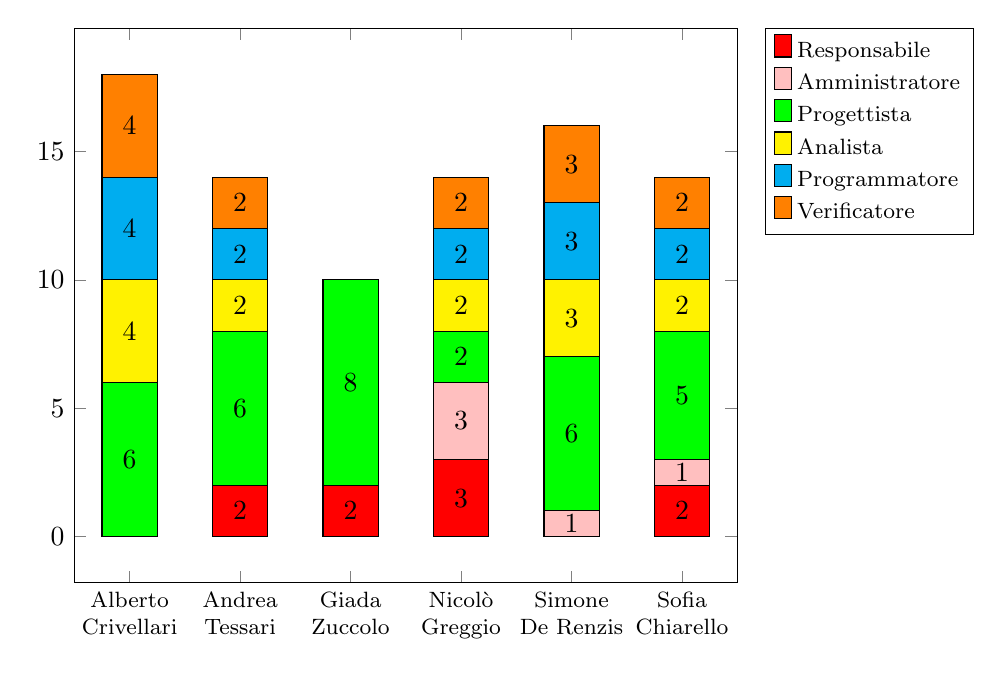
\begin{tikzpicture}
\begin{axis}[
    ybar stacked,
    width=10cm,
    bar width=0.7cm,
    %every node near coord/.style={text width=3 cm},
    nodes near coords,
     every node near coord/.append style={color=black},
    enlargelimits=0.10,
    legend style={font=\footnotesize,at={(1.2,1)},
    cells={anchor=west},
      anchor=north,legend columns=1},
    %ylabel={\#participants},
    symbolic x coords={Alberto Crivellari, Andrea Tessari, Giada Zuccolo, Nicolò Greggio, Simone De Renzis, Sofia Chiarello},
    xtick=data,
    x tick label style={font=\footnotesize,text width=1.7cm,align=center},
    ]
\addplot+[ybar,fill=red, draw=black] plot coordinates {(Alberto Crivellari,0) (Andrea Tessari,2) 
  (Giada Zuccolo,2) (Nicolò Greggio,3) (Simone De Renzis,0) (Sofia Chiarello,2) };
\addplot+[ybar,fill=pink, draw=black] plot coordinates {(Alberto Crivellari,0) (Andrea Tessari,0) 
  (Giada Zuccolo,0) (Nicolò Greggio,3) (Simone De Renzis,1) (Sofia Chiarello,1) };
\addplot+[ybar,fill=green, draw=black] plot coordinates {(Alberto Crivellari,6) (Andrea Tessari,6)
  (Giada Zuccolo,8) (Nicolò Greggio,2) (Simone De Renzis,6) (Sofia Chiarello,5) };
\addplot+[ybar,fill=yellow, draw=black] plot coordinates {(Alberto Crivellari,4) (Andrea Tessari,2) 
  (Giada Zuccolo,0) (Nicolò Greggio,2) (Simone De Renzis,3) (Sofia Chiarello,2) };
\addplot+[ybar,fill=cyan, draw=black] plot coordinates {(Alberto Crivellari,4) (Andrea Tessari,2) 
  (Giada Zuccolo,0) (Nicolò Greggio,2) (Simone De Renzis,3) (Sofia Chiarello,2) };
\addplot+[ybar,fill=orange, draw=black] plot coordinates {(Alberto Crivellari,4) (Andrea Tessari,2) 
  (Giada Zuccolo,0) (Nicolò Greggio,2) (Simone De Renzis,3) (Sofia Chiarello,2) };
\legend{Responsabile \\ Amministratore \\ Progettista \\ Analista \\ Programmatore \\ Verificatore \\}
\end{axis}
\end{tikzpicture}

\subsubsection{Prospetto economico}
Questa tabella mostra il costo per ogni ruolo all'interno del team in questa fase. Viene mostrato anche il totale. \\

\begin{tabular}{ccc}
\rowcolorhead
\headertitle{Ruolo} & \headertitle{Ore} & \headertitle{Costo(€)}\\
Responsabile & 0 & 0\\
Verificatore & 0 & 0\\
Analista & 0 & 0\\
Programmatore & 0 & 0\\
Progettista & 0 & 0\\
Totale & 0& 0\\
\end{tabular}\\

Vengono riportati i dati della tabella nel seguente grafico a torta: \\

\begin{tikzpicture}
\pie [rotate = 180, sum = auto, explode=0.1]
    {
    20/Responsabile,
	15/Verficatore,
	15/Analista,
	65/Amministratore,
	3/Programmatore,
	5/Progettista
    }
\end{tikzpicture}



\subsection{Validazione e collaudo}

\subsubsection{Prospetto orario}
Questa tabella descrive l'utilizzo della risorsa tempo (in ore) dei vari componenti del gruppo in questa fase: \\

\begin{tabular}{|l|cccccc|c|}
\hline
Nome & R &  V & An & Am & Pr & Pt & Tot(h)\\
\hline
Chiarello Sofia & 0 & 0 & 0 & 0 & 0 & 0 & 0\\
Crivellari Alberto & 0 & 0 & 0 & 0 & 0 & 0 & 0\\
De Renzis Simone & 0 & 0 & 0 & 0 & 0 & 0 & 0\\
Greggio Nicolò & 0 & 0 & 0 & 0 & 0 & 0 & 0\\
Tessari Andrea & 0 & 0 & 0 & 0 & 0 & 0 & 0\\
Zuccolo Giada & 0 & 0 & 0 & 0 & 0 & 0 & 0\\
\hline
\end{tabular}
\\
Vengono riportati i dati della tabella nel seguente istogramma: \\

\pgfplotsset{width=10cm,compat=1.17}

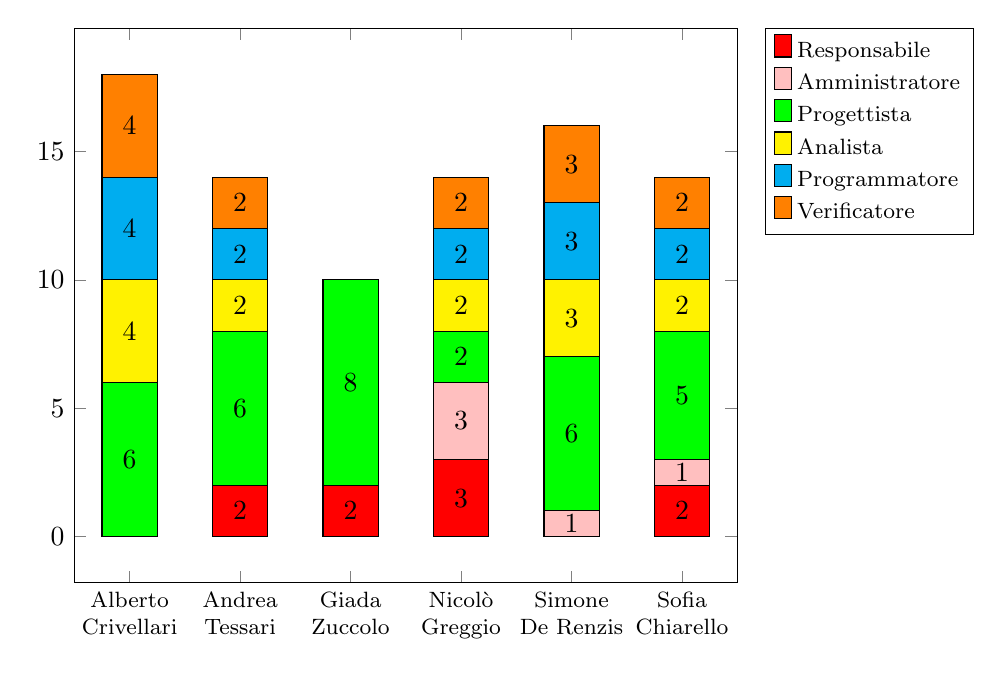
\begin{tikzpicture}
\begin{axis}[
    ybar stacked,
    width=10cm,
    bar width=0.7cm,
    %every node near coord/.style={text width=3 cm},
    nodes near coords,
     every node near coord/.append style={color=black},
    enlargelimits=0.10,
    legend style={font=\footnotesize,at={(1.2,1)},
    cells={anchor=west},
      anchor=north,legend columns=1},
    %ylabel={\#participants},
    symbolic x coords={Alberto Crivellari, Andrea Tessari, Giada Zuccolo, Nicolò Greggio, Simone De Renzis, Sofia Chiarello},
    xtick=data,
    x tick label style={font=\footnotesize,text width=1.7cm,align=center},
    ]
\addplot+[ybar,fill=red, draw=black] plot coordinates {(Alberto Crivellari,0) (Andrea Tessari,2) 
  (Giada Zuccolo,2) (Nicolò Greggio,3) (Simone De Renzis,0) (Sofia Chiarello,2) };
\addplot+[ybar,fill=pink, draw=black] plot coordinates {(Alberto Crivellari,0) (Andrea Tessari,0) 
  (Giada Zuccolo,0) (Nicolò Greggio,3) (Simone De Renzis,1) (Sofia Chiarello,1) };
\addplot+[ybar,fill=green, draw=black] plot coordinates {(Alberto Crivellari,6) (Andrea Tessari,6)
  (Giada Zuccolo,8) (Nicolò Greggio,2) (Simone De Renzis,6) (Sofia Chiarello,5) };
\addplot+[ybar,fill=yellow, draw=black] plot coordinates {(Alberto Crivellari,4) (Andrea Tessari,2) 
  (Giada Zuccolo,0) (Nicolò Greggio,2) (Simone De Renzis,3) (Sofia Chiarello,2) };
\addplot+[ybar,fill=cyan, draw=black] plot coordinates {(Alberto Crivellari,4) (Andrea Tessari,2) 
  (Giada Zuccolo,0) (Nicolò Greggio,2) (Simone De Renzis,3) (Sofia Chiarello,2) };
\addplot+[ybar,fill=orange, draw=black] plot coordinates {(Alberto Crivellari,4) (Andrea Tessari,2) 
  (Giada Zuccolo,0) (Nicolò Greggio,2) (Simone De Renzis,3) (Sofia Chiarello,2) };
\legend{Responsabile \\ Amministratore \\ Progettista \\ Analista \\ Programmatore \\ Verificatore \\}
\end{axis}
\end{tikzpicture}

\subsubsection{Prospetto economico}
Questa tabella mostra il costo per ogni ruolo all'interno del team in questa fase. Viene mostrato anche il totale. \\

\begin{tabular}{ccc}
\rowcolorhead
\headertitle{Ruolo} & \headertitle{Ore} & \headertitle{Costo(€)}\\
Responsabile & 0 & 0\\
Verificatore & 0 & 0\\
Analista & 0 & 0\\
Programmatore & 0 & 0\\
Progettista & 0 & 0\\
Totale & 0& 0\\
\end{tabular}\\

Vengono riportati i dati della tabella nel seguente grafico a torta: \\

\begin{tikzpicture}
\pie [rotate = 180, sum = auto, explode=0.1]
    {
    20/Responsabile,
	15/Verficatore,
	15/Analista,
	65/Amministratore,
	3/Programmatore,
	5/Progettista
    }
\end{tikzpicture}

\subsection{Riepilogo}

\subsubsection{Totale ore}

Questa tabella descrive l'utilizzo totale della risorsa tempo (in ore) dei vari componenti del gruppo: \\

\begin{tabular}{|l|cccccc|c|}
\hline
Nome & R &  V & An & Am & Pr & Pt & Tot(h)\\
\hline
Chiarello Sofia & 0 & 0 & 0 & 0 & 0 & 0 & 0\\
Crivellari Alberto & 0 & 0 & 0 & 0 & 0 & 0 & 0\\
De Renzis Simone & 0 & 0 & 0 & 0 & 0 & 0 & 0\\
Greggio Nicolò & 0 & 0 & 0 & 0 & 0 & 0 & 0\\
Tessari Andrea & 0 & 0 & 0 & 0 & 0 & 0 & 0\\
Zuccolo Giada & 0 & 0 & 0 & 0 & 0 & 0 & 0\\
\hline
\end{tabular}
\\
Vengono riportati i dati della tabella nel seguente istogramma: \\

\pgfplotsset{width=10cm,compat=1.17}

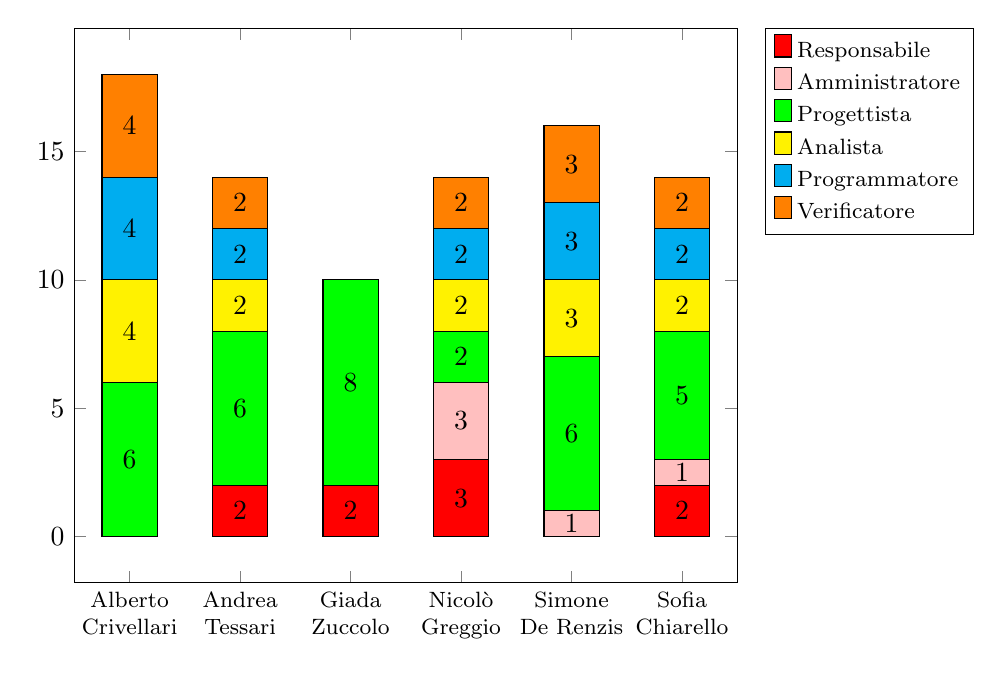
\begin{tikzpicture}
\begin{axis}[
    ybar stacked,
    width=10cm,
    bar width=0.7cm,
    %every node near coord/.style={text width=3 cm},
    nodes near coords,
     every node near coord/.append style={color=black},
    enlargelimits=0.10,
    legend style={font=\footnotesize,at={(1.2,1)},
    cells={anchor=west},
      anchor=north,legend columns=1},
    %ylabel={\#participants},
    symbolic x coords={Alberto Crivellari, Andrea Tessari, Giada Zuccolo, Nicolò Greggio, Simone De Renzis, Sofia Chiarello},
    xtick=data,
    x tick label style={font=\footnotesize,text width=1.7cm,align=center},
    ]
\addplot+[ybar,fill=red, draw=black] plot coordinates {(Alberto Crivellari,0) (Andrea Tessari,2) 
  (Giada Zuccolo,2) (Nicolò Greggio,3) (Simone De Renzis,0) (Sofia Chiarello,2) };
\addplot+[ybar,fill=pink, draw=black] plot coordinates {(Alberto Crivellari,0) (Andrea Tessari,0) 
  (Giada Zuccolo,0) (Nicolò Greggio,3) (Simone De Renzis,1) (Sofia Chiarello,1) };
\addplot+[ybar,fill=green, draw=black] plot coordinates {(Alberto Crivellari,6) (Andrea Tessari,6)
  (Giada Zuccolo,8) (Nicolò Greggio,2) (Simone De Renzis,6) (Sofia Chiarello,5) };
\addplot+[ybar,fill=yellow, draw=black] plot coordinates {(Alberto Crivellari,4) (Andrea Tessari,2) 
  (Giada Zuccolo,0) (Nicolò Greggio,2) (Simone De Renzis,3) (Sofia Chiarello,2) };
\addplot+[ybar,fill=cyan, draw=black] plot coordinates {(Alberto Crivellari,4) (Andrea Tessari,2) 
  (Giada Zuccolo,0) (Nicolò Greggio,2) (Simone De Renzis,3) (Sofia Chiarello,2) };
\addplot+[ybar,fill=orange, draw=black] plot coordinates {(Alberto Crivellari,4) (Andrea Tessari,2) 
  (Giada Zuccolo,0) (Nicolò Greggio,2) (Simone De Renzis,3) (Sofia Chiarello,2) };
\legend{Responsabile \\ Amministratore \\ Progettista \\ Analista \\ Programmatore \\ Verificatore \\}
\end{axis}
\end{tikzpicture}

\subsubsection{Prospetto economico}
Questa tabella mostra il costo totale per ogni ruolo all'interno del team. Viene mostrato anche il totale. \\

\begin{tabular}{ccc}
\rowcolorhead
\headertitle{Ruolo} & \headertitle{Ore} & \headertitle{Costo(€)}\\
Responsabile & 0 & 0\\
Verificatore & 0 & 0\\
Analista & 0 & 0\\
Programmatore & 0 & 0\\
Progettista & 0 & 0\\
Totale & 0& 0\\
\end{tabular}\\

Vengono riportati i dati della tabella nel seguente grafico a torta: \\

\begin{tikzpicture}
\pie [rotate = 180, sum = auto, explode=0.1]
    {
    20/Responsabile,
	15/Verficatore,
	15/Analista,
	65/Amministratore,
	3/Programmatore,
	5/Progettista
    }
\end{tikzpicture}



\subsubsection{Ore rendicontate}
\subsubsection{Lavoro Rendicontato}
Questa tabella descrive il numero di ore redicontate di ogni componente del gruppo: \\

\begin{tabular}{|l|cccccc|c|}
\hline
Nome & R &  V & An & Am & Pr & Pt & Tot(h)\\
\hline
Chiarello Sofia & 0 & 0 & 0 & 0 & 0 & 0 & 0\\
Crivellari Alberto & 0 & 0 & 0 & 0 & 0 & 0 & 0\\
De Renzis Simone & 0 & 0 & 0 & 0 & 0 & 0 & 0\\
Greggio Nicolò & 0 & 0 & 0 & 0 & 0 & 0 & 0\\
Tessari Andrea & 0 & 0 & 0 & 0 & 0 & 0 & 0\\
Zuccolo Giada & 0 & 0 & 0 & 0 & 0 & 0 & 0\\
\hline
\end{tabular}
\\
Vengono riportati i dati della tabella nel seguente istogramma: \\

\pgfplotsset{width=10cm,compat=1.17}

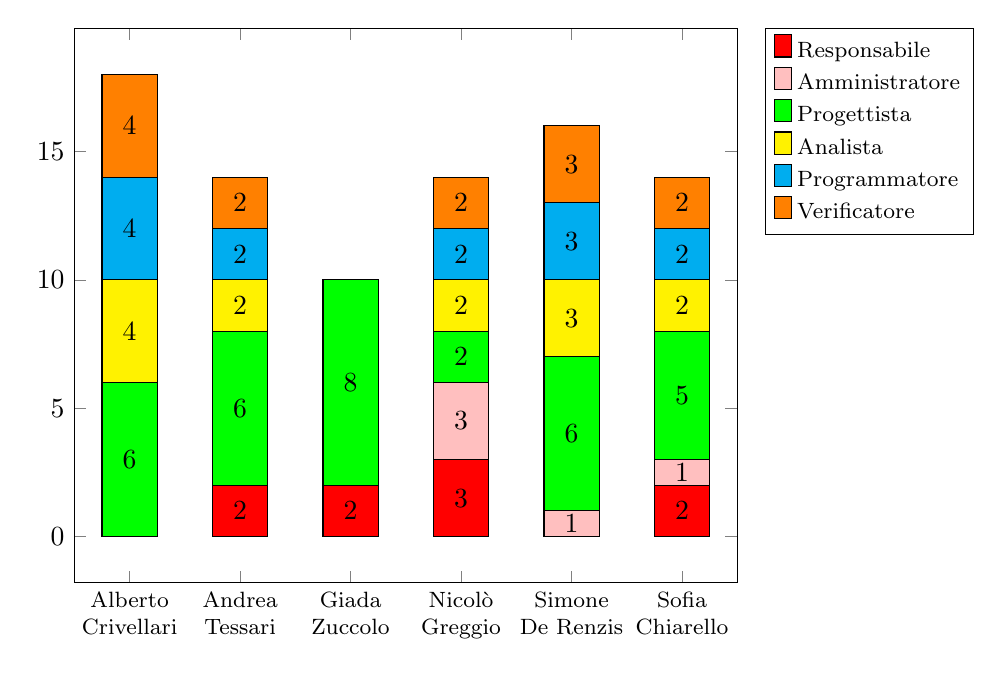
\begin{tikzpicture}
\begin{axis}[
    ybar stacked,
    width=10cm,
    bar width=0.7cm,
    %every node near coord/.style={text width=3 cm},
    nodes near coords,
     every node near coord/.append style={color=black},
    enlargelimits=0.10,
    legend style={font=\footnotesize,at={(1.2,1)},
    cells={anchor=west},
      anchor=north,legend columns=1},
    %ylabel={\#participants},
    symbolic x coords={Alberto Crivellari, Andrea Tessari, Giada Zuccolo, Nicolò Greggio, Simone De Renzis, Sofia Chiarello},
    xtick=data,
    x tick label style={font=\footnotesize,text width=1.7cm,align=center},
    ]
\addplot+[ybar,fill=red, draw=black] plot coordinates {(Alberto Crivellari,0) (Andrea Tessari,2) 
  (Giada Zuccolo,2) (Nicolò Greggio,3) (Simone De Renzis,0) (Sofia Chiarello,2) };
\addplot+[ybar,fill=pink, draw=black] plot coordinates {(Alberto Crivellari,0) (Andrea Tessari,0) 
  (Giada Zuccolo,0) (Nicolò Greggio,3) (Simone De Renzis,1) (Sofia Chiarello,1) };
\addplot+[ybar,fill=green, draw=black] plot coordinates {(Alberto Crivellari,6) (Andrea Tessari,6)
  (Giada Zuccolo,8) (Nicolò Greggio,2) (Simone De Renzis,6) (Sofia Chiarello,5) };
\addplot+[ybar,fill=yellow, draw=black] plot coordinates {(Alberto Crivellari,4) (Andrea Tessari,2) 
  (Giada Zuccolo,0) (Nicolò Greggio,2) (Simone De Renzis,3) (Sofia Chiarello,2) };
\addplot+[ybar,fill=cyan, draw=black] plot coordinates {(Alberto Crivellari,4) (Andrea Tessari,2) 
  (Giada Zuccolo,0) (Nicolò Greggio,2) (Simone De Renzis,3) (Sofia Chiarello,2) };
\addplot+[ybar,fill=orange, draw=black] plot coordinates {(Alberto Crivellari,4) (Andrea Tessari,2) 
  (Giada Zuccolo,0) (Nicolò Greggio,2) (Simone De Renzis,3) (Sofia Chiarello,2) };
\legend{Responsabile \\ Amministratore \\ Progettista \\ Analista \\ Programmatore \\ Verificatore \\}
\end{axis}
\end{tikzpicture}

\subsubsection{Prospetto economico}
Questa tabella mostra il costo totale rendicontato per ogni ruolo all'interno del team. Viene mostrato anche il totale. \\

\begin{tabular}{ccc}
\rowcolorhead
\headertitle{Ruolo} & \headertitle{Ore} & \headertitle{Costo(€)}\\
Responsabile & 0 & 0\\
Verificatore & 0 & 0\\
Analista & 0 & 0\\
Programmatore & 0 & 0\\
Progettista & 0 & 0\\
Totale & 0& 0\\
\end{tabular}\\

Vengono riportati i dati della tabella nel seguente grafico a torta: \\

\begin{tikzpicture}
\pie [rotate = 180, sum = auto, explode=0.1]
    {
    20/Responsabile,
	15/Verficatore,
	15/Analista,
	65/Amministratore,
	3/Programmatore,
	5/Progettista
    }
\end{tikzpicture}


\subsection{Conclusione}
Il progetto è venuto a costare NNN €, tenendo conto solamente delle ore rendicontate.
